\lohead{Florian Greistorfer}
\chapter{Webserver und Client}

\section{Begriffserklärungen}
\label{sec:begriffserklaerung}

\subsection{Server}
\label{sec:begrr-server}
Ein Programm, der oder das Zugriff auf eine Resource oder einen Dienst in einem Netzwerk ermöglicht

\subsection{Client}
\label{sec:begrr-client}
Ein Programm, der oder das auf einen Server zugreift

\section{Anforderungen}
\label{sec:anforderungen}

\subsection{Webserver}
\label{sec:anf-server}
Auf der Katzenfütterungsanlage läuft ein Webserver, der es ermöglicht, dass der Benutzer das Gerät über das Internet erreichen kann. Hauptaufgaben des Servers sind dabei, Daten bereitzustellen, zu verabeiten und zu speichern und den Webclient zur Verfügung zu stellen.

\subsection{Client}
\label{sec:anf-client}
Der Client soll dem Benutzer ermöglichen, die Katzenfütterungsanlage über einen Webbrowser zu steuern. Ein Benutzername und ein Passwort sind erforderlich, damit man das Gerät bedienen kann. Das Design soll eindeutig und übersichtlich gehalten sein. Auf der Startseite sollen die eingestellten Fütterungszeiten zu sehen sein und eine allgemeine Übersicht. Über eine Navigationsleiste sollen die weiteren Seiten erreichbar sein:

\begin{itemize}
\item[•]Fütterrungszeiten
\item[•]Positionsinfo
\item[•]Geräteinfo
\item[•]Update
\end{itemize}

\section{Voruntersuchung}
\label{sec:voruntersuchung}

\subsection{HTTP/HTTPS}
\label{sec:vor-http}
Das \ac{HTTP}\footnote{Weitere Informationen zu \ac{HTTP} unter \url{https://developer.mozilla.org/de/docs/Web/HTTP}} ist der Kommunikationsstandart auf dem das Internet basiert. Eine HTTP Session wird über eine Anfrage über das \ac{TCP} an einen Server auf den Port 80 initiiert. Der Server, der auf diesem Port auf eine Anfrage wartet sendet eine Statusmeldung wie z.B. \inlinecode{bash}{HTTP/1.1 200 OK} und eventuell eine eigene Nachricht zurück. Diese Nachricht ist meist die angeforderte Resource oder eine Fehlermeldung. \ac{HTTPS} ist die verschlüsselte Version von \ac{HTTP}. Die meist gebrauchten Anfragen sind:

\begin{itemize}
\item[•] \textbf{GET}: Fordert eine Repräsentation der Ressource an. Ein GET Request darf nur Daten abfragen und darf keinen anderen Einfluss haben.
\item[•] \textbf{PUT}: Fordert das Speichern der Daten, die sich im Request-Body befinden, an. Wenn bereits eine Ressource an der angegebenen \ac{URI} existiert, so wird diese aktualisiert, sonst wird die Resource erstellt.
\item[•] \textbf{POST}: Fordert das Speichern der Daten, die sich im Request-Body befinden, unter der angegebenen \ac{URI} an. 
\item[•] \textbf{DELETE}: Fordert das Löschen der Ressource unter der angegebenen \ac{URI} an.
\end{itemize}

\subsection{JavaScript}
\label{sec:vor-js}
JavaScript ist die Programmiersprache des Internets. Jeder herkömmliche Browser ist in der Lage, JavaScript auszuführen. Mit JavaScript ist es möglich, das Aussehen einer Webseite während der Laufzeit zu ändern, Dinge zu entfernen, hinzufügen und animieren. JavaScript ist heute eine objektorientierte Sprache. Es hebt sich von anderen Sprachen vor allem dadurch ab, dass die Datentypen von Variable nicht fix sind. Das bedeutet, wenn eine Variable den Datentyp \textit{number} hat und es wird ein String angehängt, verändert sich der Datentyp automatisch auf \textit{string}.

\subsection{Node.js}
\label{sec:vor-node}
Node.js ist eine Laufzeitumgebung, die es ermöglicht, dass Javascript direkt auf einem Rechner ausgeführt werden kann. Node.js kommt mit dem \ac{npm}. Mithilfe diesem Tools ist es möglich, Module zu installieren, updaten, löschen und veröffentlichen. Diese Module werden im Ordner \textit{/node\_modules} installiert und in der Datei \textit{package.json} unter \textit{dependencies}, oder mit der option \inlinecode{bash}{--save-dev} unter \textit{dev-dependencies} eingetragen. Ein neues Projekt erstellt man mit \inlinecode{bash}{npm init}. Dieses Tool erstellt die Datei \textit{package.json}, in der alle Abhängigkeiten und Informationen über das Projekt stehen. Wenn man ein Projekt kopiert, braucht man den \textit{/node\_modules} Ordner nicht mit kopieren. Man muss nur im Zielordner einmal \inlinecode{bash}{npm install} aufrufen.

\subsection{TypeScript}
\label{sec:vor-ts}
TypeScript ist eine, von Microsoft entwickelte, Weiterentwicklung von JavaScript. Das bedeutet, jeder gültige JavaScript Code ist auch ein gültiger TypeScript Code. TypeScript wird vom TypeScript Compiler in sauberes JavaScript übersetzt. TypeScript ist sehr gut für größere Anwendungen geeignet. Typescript hat strenge Datentypen, Klassen und Vererbung. Die Datentypen von TypeScript sind:

\begin{itemize}
\item[•] \textbf{string}: eine Unicode codierte Zeichenkette
\item[•] \textbf{number}: eine vorzeichenbehaftete Gleitkommazahl, kann auch hexadezimal, octal oder binär sein
\item[•] \textbf{boolean}: true oder false
\item[•] \textbf{array}: eine Liste von Elementen des gleichen Datentyps
\item[•] \textbf{tuple}: eine Liste von Elementen unterschiedlichen Datentyps deren Anzahl bekannt ist
\item[•] \textbf{enum}: eine Möglichkeit, numerischen Werten Namen zu geben
\item[•] \textbf{any}: Datentyp unbekannt, wird behandelt wie in JavaScript
\item[•] \textbf{void}: kein Datentyp, meist Rückgabewert bei Funktionen
\item[•] \textbf{null}: leerer Wert, kann allen anderen zugewiesen werden
\item[•] \textbf{undefined}: kein Wert, kann allen anderen zugewiesen werden
\item[•] \textbf{never}: wenn ein Wert niemals auftreten kann z.B. eine Funktion die immer einen Fehler produziert
\end{itemize}

Damit JavaScript Module von TypeScript verwendet werden können, benötigen sie sogenannte Type Annotations. Diese können bei den meisten bekannteren Modulen über den \ac{npm} installiert werden. Diese Pakete haben den Namenspräfix \textit{@types/}, das bedeutet, dass zum Beispiel die Type Annotations des Express Moduls über \inlinecode{bash}{npm install --save-dev @types/express} installiert werden können. Sollten keine Type Annotations für ein Modul vorhanden sein, muss man diese selbst erstellen.

\subsection{express}
\label{sec:vor-express}
Express ist ein Javascript Modul, dass auf dem Node.js Modul \textit{http} bzw \textit{https} aufbaut. In diesen Modulen ist bereits alles enthalten, dass benötigt wird, um einen Webserver zu programmieren. Express nimmt uns die meiste Arbeit ab und bietet viele weitere Möglichkeiten.

\subsection{JSON}
\label{sec:vor-json}
\ac{JSON} ist die Textrepräsentation eines JavaScript Objekts\footnote{Weiter Informationen zu \ac{JSON} unter \url{https://www.json.org/}}. Die möglichen Datentypen sind:

\begin{itemize}
\item[•] \textbf{string}: 0 oder mehrere unicode Zeichen innerhalb Doppelhochkommas
\item[•] \textbf{boolean}: true oder false
\item[•] \textbf{number}: Eine vorzeichenbehaftete Zahl, die auch die E Notation unterstützt z.B. 0.2E4 (=2000)
\item[•] \textbf{Array}: Eine geordnete Liste von 0 oder mehreren Werten innerhalb eckiger Klammern, Elemente sind getrennt durch Kommas.
\item[•] \textbf{Object}: Eine ungeordnete Sammlung von Name-Wert-Paaren, wo die Namen, die auch Keys genannt werden, Strings sind. Jeder Key sollte eindeutig sein. Innerhalb geschwungener Klammern. Paare sind durch Komma getrennt
\item[•] \textbf{null}: Ein leerer Wert
\end{itemize}

\begin{lstlisting}[style=JSON,caption=\ac{JSON} Beispiel]
{
	"Object": {	
		"string": "name",
		"number": 10E5,
		"boolean": true,
		"Array": [
			{
				"string": "wert",
				"number": 1
			},
			{
				"string": "wert",
				"number": 2
			}
		]
	}
}
\end{lstlisting}

\subsection{JSON Web Token}
\label{sec:vor-jwt}
\ac{JWT} ist ein JSON-basierter, offener Standard für das erstellen von Access Tokens. Mithilfe eines \ac{JWT} kann ein Client sich ausweisen. Ein \ac{JWT} wird vom Server entweder mit einem Secret oder seinem privaten Schlüssel signiert. Dadurch können Server und Client beide überprüfen, ob der Token legitim ist. Ein \ac{JWT} besteht aus drei Teilen. Dem Header, der Payload und der Signature. Im Header steht der fürs Verschlüsseln der Signatur benutzte Algorithmus z.B: \inlinecode{JSON}{\{"alg":"RS256","typ":"JWT"\}}. Im Payload stehen die Daten, die entweder den Client ausweisen oder ähnliche Information. Beispiel: \inlinecode{JSON}{\{"user": "cat", "iat": 1520875121, "exp": 1520911121\}} \textit{iat} bedeutet \textit{issued at} und sagt aus, wann der Token generiert wurde. In der Signature steht der Key, der unsignierte Token, das ist der Header und die Payload Base64 codiert, und die Signatur. Alle drei Teile werden Base64 codiert und mittels Punkt voneinander getrennt.

\subsection{MongoDB}
\label{sec:vor-mongo}
MongoDB ist eine schemenlose Datenbank. Schemenlos bedeutet, dass die Datenbank, im Vergleich zu schemenbehafteten Datenbanken, keine klare Strukturierung benötigt. Einer schemenlosen Datenbank kann man einfach Daten geben und wieder abfragen. Eine schemenbehaftete Datenbank ist in Zeilen und Spalten unterteilt. Diese müssen vorher feststehen. Da Raspian, das Betriebssystem vom Raspberry Pi, nur 32 Bit ist und MongoDB ab Version 3 nur mehr in 64 Bit erhältlich ist, mussten wir auf eine ältere Version wechseln. Die Verbindung der MongoDB Datenbank erfolgt über einen Driver. Der Driver muss mit der Datenbankversion übereinstimmen. MongoDB ist ein \ac{DBMS}, das bedeutet, ein Server läuft auf dem Port 27017, über den alle Datenbanken im System erreichbar sind z.B. die Datenbank \textit{fuettr} ist über \inlinecode{bash}{localhost:27017/fuettr} erreichbar. Eine Gruppe von Daten nennt man Collection. Zugriff auf die Datenbank erfolgt serverseitig wie folgt:

\begin{lstlisting}[caption=Verbinden mit dem \ac{DBMS},style=TS]
const dbServer = await mongodb.MongoClient.connect(url);
\end{lstlisting}

\begin{lstlisting}[caption=Auswählen der Datenbank,style=TS]
const dbFuettr = await dbServer.db('fuettr');
\end{lstlisting}

\begin{lstlisting}[caption=Auswählen der Collection,style=TS]
const collTimes = await dbFuettr.collection('data_times');
\end{lstlisting}

\begin{lstlisting}[caption=Auslesen aller Datensätze mit einem Identifier,style=TS]
const Times = await this._times.find({ identifier: 'Times' }).toArray();
\end{lstlisting}

\begin{lstlisting}[caption=Überschreiben eines Datensatzes mit einem Identifier,style=TS]
this._times.updateOne({ identifier: 'Times' }, { $set: times });
\end{lstlisting}

\subsection{DOM}
\label{sec:vor-dom}
Das \ac{DOM} ist die Objektrepräsentation des \ac{HTML} Dokuments. Durch das \ac{DOM} kann eine JavaScript Anwendung \ac{HTML} Elemente ändern, entfernen, und hinzufügen, \ac{HTML} Attribute ändern, entfernen und hinzufügen und \ac{CSS} Styles ändern. Das \ac{DOM} wird vom Browser beim Laden der Website erstellt. 

\subsection{Angular 2/4}
\label{sec:vor-angular}
Angular ist ein TypeScript Framework, das aus dem Javascript-Framework AngularJS weiterentwickelt wurde. Es wird von Google entwickelt. Angular ist gegliedert in Module. Die grobe Struktur wird in der Abbildung \ref{Angular Struktur} dargestellt.

\begin{figure}[H]
      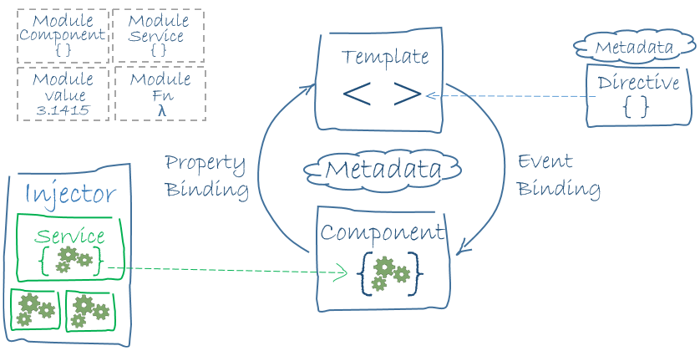
\includegraphics[width=1\textwidth]{Bilder/Greistorfer/Angular}
      \caption{Angular Struktur}
      \label{Angular Struktur}
\end{figure}

\subsubsection{Modules}
\label{sec:ang-modules}
Jede Angular App ist in \textit{Module}s gegliedert. \textit{Module}s fassen meist ähnliche Funktionen zusammen. Jede App muss mindestens ein \textit{Module} enthalten. Dies heißt standardmäßig \textit{AppModule}. Ein \textit{Module} ist die größte Einheit einer Angular App.  Ein \textit{Module} kann folgende Komponenten beinhalten:

\begin{itemize}
\item[•]Services
\item[•]Andere Module
\item[•]View Classes
\begin{itemize}
\item[-]Components
\item[-]Directives
\item[-]Pipes
\end{itemize}
\end{itemize}

\subsubsection{Libraries}
\label{sec:ang-libraries}
Eine Angular Library ist ein Modul, das \textit{decorator} und \textit{Modules} exportiert. Diese können von \textit{Components} und \textit{Modules} importiert werden. Der Name jeder Angular library beginnt mit \textit{@angular}. Angular libraries können mit dem \ac{npm} installiert werden.

\subsubsection{Components}
\label{sec:ang-components}
Ein \textit{Component} kontrolliert einen Teil des Bildschirms, den sogenannten \textit{view}. Die Logik des \textit{Component}s wird in einer Klasse definiert. Die Klasse interagiert mit dem \textit{view} durch eine \ac{API} von Eigenschaften und Methoden.

\paragraph*{Lifecycle Hooks}\mbox{}\\
Ein Lebenszyklus in Angular ist immer der Lebenszyklus des jeweiligen \textit{Components}. Ein \textit{Component} kann erstellt, verändert und zerstört werden. Zu jedem Stadium gibt es eine Methode, die automatisch je nach Stadium von Angular aufgerufen werden. Die am häufigsten verwendeten sind:

\begin{itemize}
\item[•] \textbf{OnInit()}: Wird aufgerufen, wenn der \textit{Component} erstellt wird. Die dazugehörige Methode ist \inlinecode{TS}{ngOnInit()}. Zeitaufwendige Operationen sollten hier aufgerufen werden, anstatt im constructor, da das den Erzeugungsvorgang verlangsamen würden.
\item[•] \textbf{OnDestroy()}: Wird aufgerufen, wenn der \textit{Component} zerstört wird. Die dazugehörige Methode ist \inlinecode{TS}{ngOnDestroy()}. Hier sollten alle laufenden Prozesse, wie Intervals und Callbacks beendet werden.
\item[•] \textbf{OnChanges()/DoCheck()}: Werden aufgerufen, wenn sich irgentetwas an der \textit{Component} ändert. Die dazugehörige Methoden sind \inlinecode{TS}{ngOnChanges()} und \inlinecode{TS}{ngDoCheck()}.
\end{itemize}

Alle Lifecycle Hooks müssen von der Klasse mit \inlinecode{TS}{implements} implementiert und von \textit{@angular/core} importiert werden.

\subsubsection{Templates}
\label{sec:ang-templates}
Das Aussehen des \textit{view}s wird in einem \textit{Template} definiert. Ein \textit{Template} ist eine \ac{HTML} Datei, mit Angular's Template Syntax. Das bedeutet, dass einige Zusatzbefehle vorkommen können. Beispiele hierfür sind:

\begin{itemize}
\item[•]*ngFor
\item[•]*ngIf
\item[•]\{\{variable\}\}
\item[•](click)
\item[•][variable]
\item[•]<app-route>
\end{itemize}

Die meisten Zusatzbefehle werden für \textit{Data Binding} verwendet.

\mbox{}
\begin{wrapfigure}{l}{0.5\textwidth}
\vspace{-50pt}
  \begin{center}
    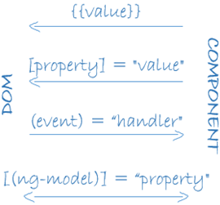
\includegraphics[width=0.4\textwidth]{Bilder/Greistorfer/databinding}
  \end{center}
  \caption{Angular Databinding}
  \label{Angular Databinding}
  \vspace{0pt}
\end{wrapfigure}
\vspace{-40pt}
\subsubsection{Data binding}
\label{sec:ang-data-binding}
Ohne Framework wäre der Programmierer dafür verantwortlich, sicherzustellen, dass Daten in \ac{HTML} Elemente geschrieben werden und dass auf Benutzerinteraktionen reagiert wird. Das ist aufwendig, Fehleranfällig und schwer zu lesen. Angulars Lösung dafür nennt sich \textit{data binding}. Der Programmierer muss nur mehr im \ac{HTML} Template Angular mitteilen, wie die beiden Seiten verbunden werden sollen. In der Abbilung \ref{Angular Databinding} sind die vier möglichen Arten von \textit{data binding} dargestellt. Jede Art hat eine Richtung, vom \ac{DOM} zum \ac{DOM} oder in beide Richtungen.

\begin{itemize}
\item[•] \inlinecode{Html}{<span>\{\{variable\}\}</span>} Der Wert der Variable in den Klammern wird anstelle des Klammerausdrucks dargestellt. Wenn sich der Wert ändert, ändert sich auch der Wert im \ac{DOM}
\item[•] \inlinecode{Html}{<span [hidden]="hide"></span>} übergibt den Wert in der angegebenen Variable in das angegebene Attribut
\item[•] \inlinecode{Html}{<span (click)="clicked(\$event)"></span>} ruft die angegebene Methode auf, wenn das angegebene Event auftritt.
\item[•] \inlinecode{Html}{<input [(ngModel)]="variable">} der Wert im Eingabefeld und in der Variable sind voneinander abhängig, ändert sich der eine, so ändert sich der andere zum gleichen
\end{itemize}

\subsubsection{Services}
\label{sec:ang-services}
Services sind Klassen, die eine Aufgabe erfüllen, unabhängig von allem anderen. Sie werden vor allem verwendet, wenn eine Aufgabe etwas Zeit erfordert, wie z.B. eine Serveranfrage. Services bieten auch die Möglichkeit, dass \textit{Components} Zugriff auf eine gemensame Variable haben, da Angular keine globalen Variablen hat. Services müssen vom \textit{Dependency Injector} injiziert werden. Der \textit{Dependency Injector} indiziert alle Abhängigkeiten in eine \textit{Component}.

\subsection{Angular CLI}
\label{sec:vor-angular-cli}
Das Angular \ac{CLI} ist ein JavaScript Modul, das über den \ac{npm} installiert werden kann. Mithilfe des \ac{CLI} ist das erstellen und übersetzen von Angular Anwendungen um vieles erleichtert. Ein neues Projekt erstellt man mit \inlinecode{bash}{ng new <projektname>} und übersetzt wird mit \inlinecode{bash}{ng build}. Mit der Option \inlinecode{bash}{--prod} wird die Anwendung kompakter und für den Einsatz im produktiven Umfeld übersetzt.

\subsection{Bootstrap}
\label{sec:vor-bootstrap}
Bootstrap ist eine CSS Bibliothek, die die Möglichkeit bietet, bereits vorgefertigte Komponenten auf unserer Website zu verwenden. An erster Stelle stehen bei Bootstrap responsive Design und Mobilgeräte. Responsive bedeutet, dass die Elemente sich an die breite des Bildschirms anpassen. Dadurch erspart man sich als nicht sehr designaffiner Programmierer viel Arbeit. Auf der offiziellen Bootstrap Website kann man außerdem verschiedene Themes auswählen. Bootstrap wurde von Twitter entwickelt und ist entweder über den \ac{npm} oder über Bootstraps eigenes \ac{CDN} erhältlich.

\section{Umsetzung}
\label{sec:umsetzung}

\subsection{Projektstruktur}
\label{sec:ums-projektstruktur}
\dirtree{%
.1 Webserver.
.2 server.
.3 dist.
.3 keys.
.3 node\_modules.
.3 public.
.3 src.
.4 views.
.2 ngx.
.3 dist.
.3 e2e.
.3 node\_modules.
.3 src.
.4 app.
.5 components.
.5 services.
.4 assets.
.4 environments.
.4 i18n.
}

Das Projekt ist so strukturiert, dass eine klare Trennung zwischen Client und Server herrscht.
\paragraph*{Server} Im \textit{keys} Ordner befinden sich der öffentliche und private Schlüssel, die vom install Script erstellt werden. Im \textit{public} Ordner befinden sich die Ressourcen, die direkt vom Server gesendet werden, z.B. Fehlermeldungsseiten. Im \textit{src} Ordner sind die TypeScript Arbeitsdateien. Diese werden in den \textit{dist} Ordner übersetzt.
\paragraph*{Client} Der Client Ordner hat den Namen \textit{ngx}, dass sagt aus, es ist ein Angular Projekt, die Angular Version ist aber egal. Im \textit{src} Ordner befinden sich alle Dateien, die das Angular \ac{CLI} benötigt, um die Anwendung zu bauen. Im \textit{assets} Ordner befinden sich alle Ressourcen, die die Anwendung benötigt, wie z.B. Bilder. Im Ordner \textit{i18n} befinden sich die Dateien, die das \ac{CLI} braucht, um die Anwendung in mehrere Sprachen zu übersetzen. Im \textit{app} Ordner befindet sich die eigentlich Anwendung. Die Anwendung ist klar getrennt in den Ordner \textit{components} und \textit{services}.

\subsection{Client}
\label{sec:ums-client}

\subsubsection{Design}
\label{sec:ums-client-design}
Das Design sollte übersichtlich und einfach gestaltet werden. Der Benutzer soll auf den ersten Blick die wichtigsten Funktionen und Informationen erkennen können. \\

\begin{wrapfigure}{r}{0.7\textwidth}
\vspace{-10pt}
  \begin{center}
    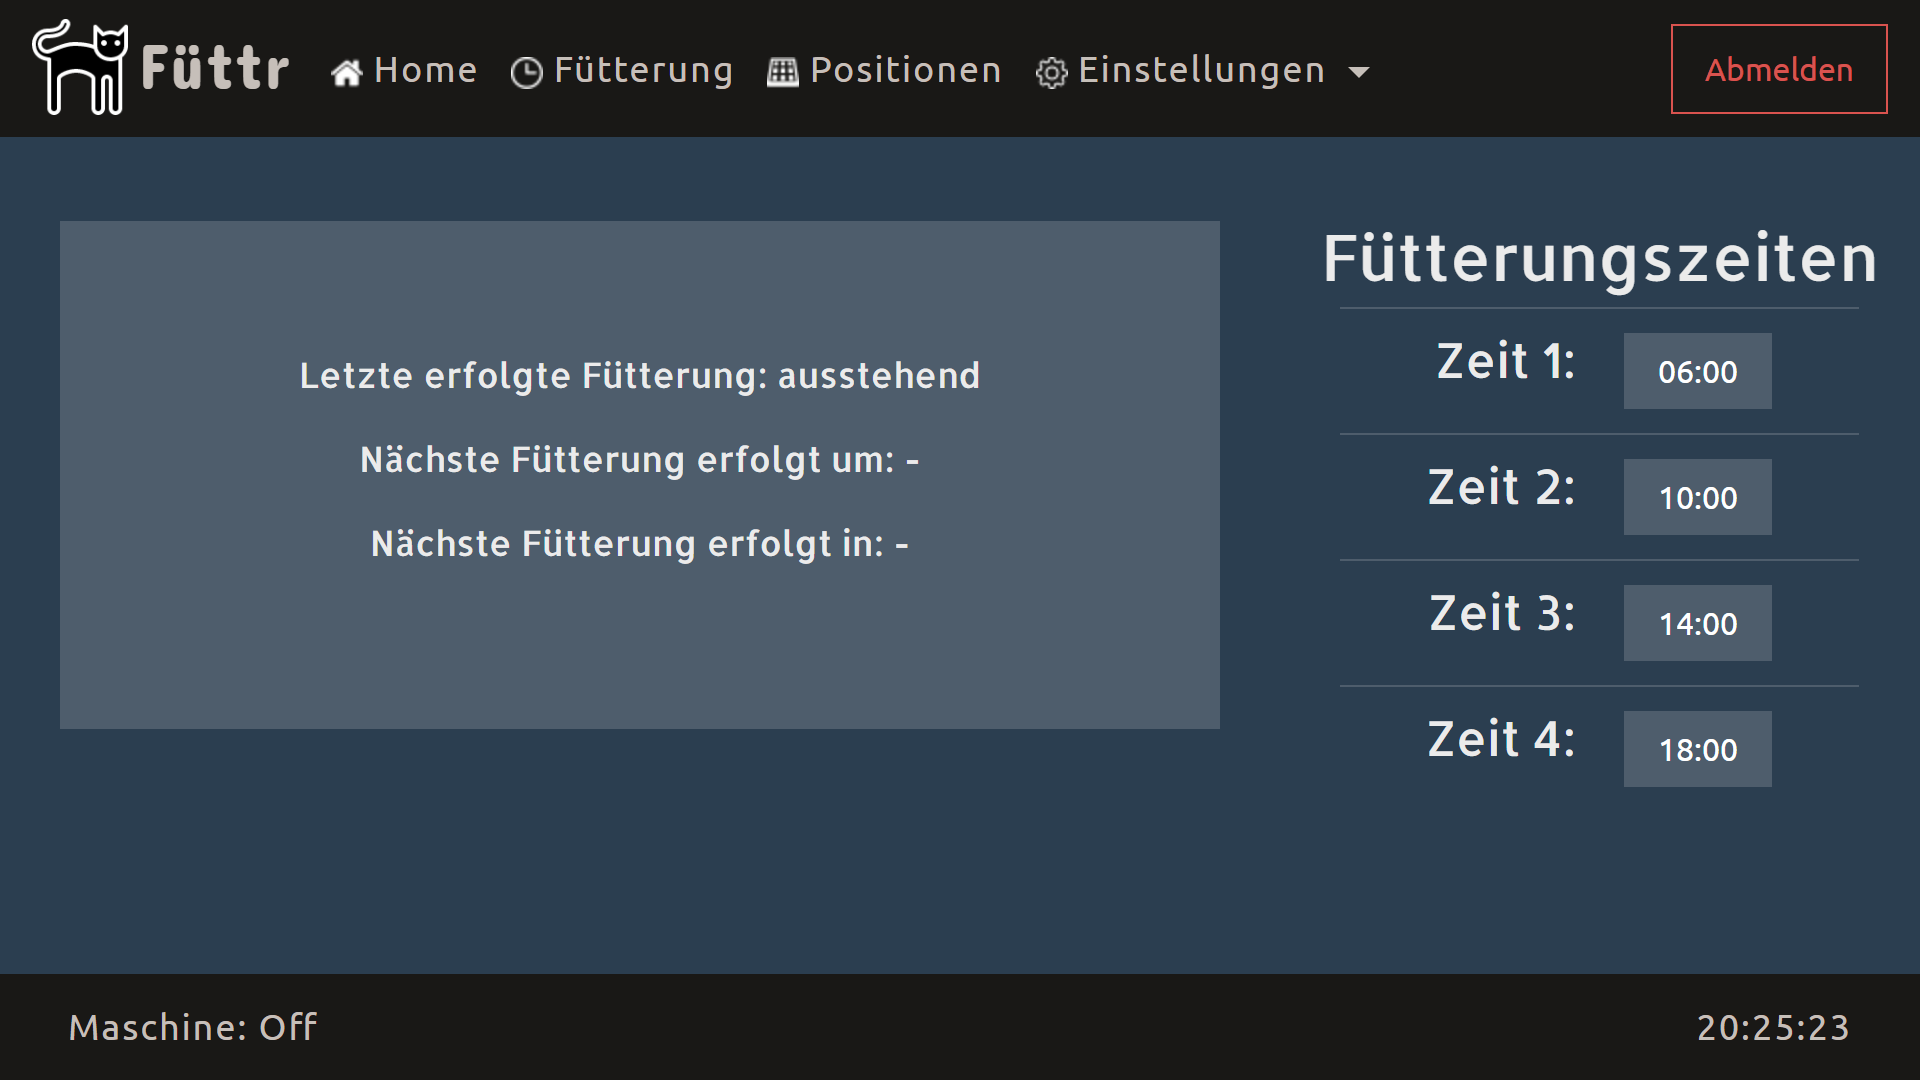
\includegraphics[width=0.65\textwidth]{Bilder/Greistorfer/Home}
  \end{center}
  \caption{Startseite}
  \label{Startseite}
  \vspace{-10pt}
\end{wrapfigure}

Auf der Startseite sind alle wichtigen Informationen übersichtlich dargestellt. Auf der linken Seite werden die Uhrzeit der letzten erfolgreichen Fütterung, die Zeit der nächsten Fütterung und die Zeit bis zur nächsten Fütterung dargestellt. Darunter werden Fehler und Warnungen, falls welche auftreten sollten, angezeigt. Da unbekannt ist, wie viele Fehler und Warnungen auftreten, werden diese in einem *ngFor aufgelistet. Auf der rechten Seite sind die aktiven Fütterungszeiten aufgelistet. \newpage

\begin{wrapfigure}{r}{0.7\textwidth}
\vspace{-10pt}
  \begin{center}
    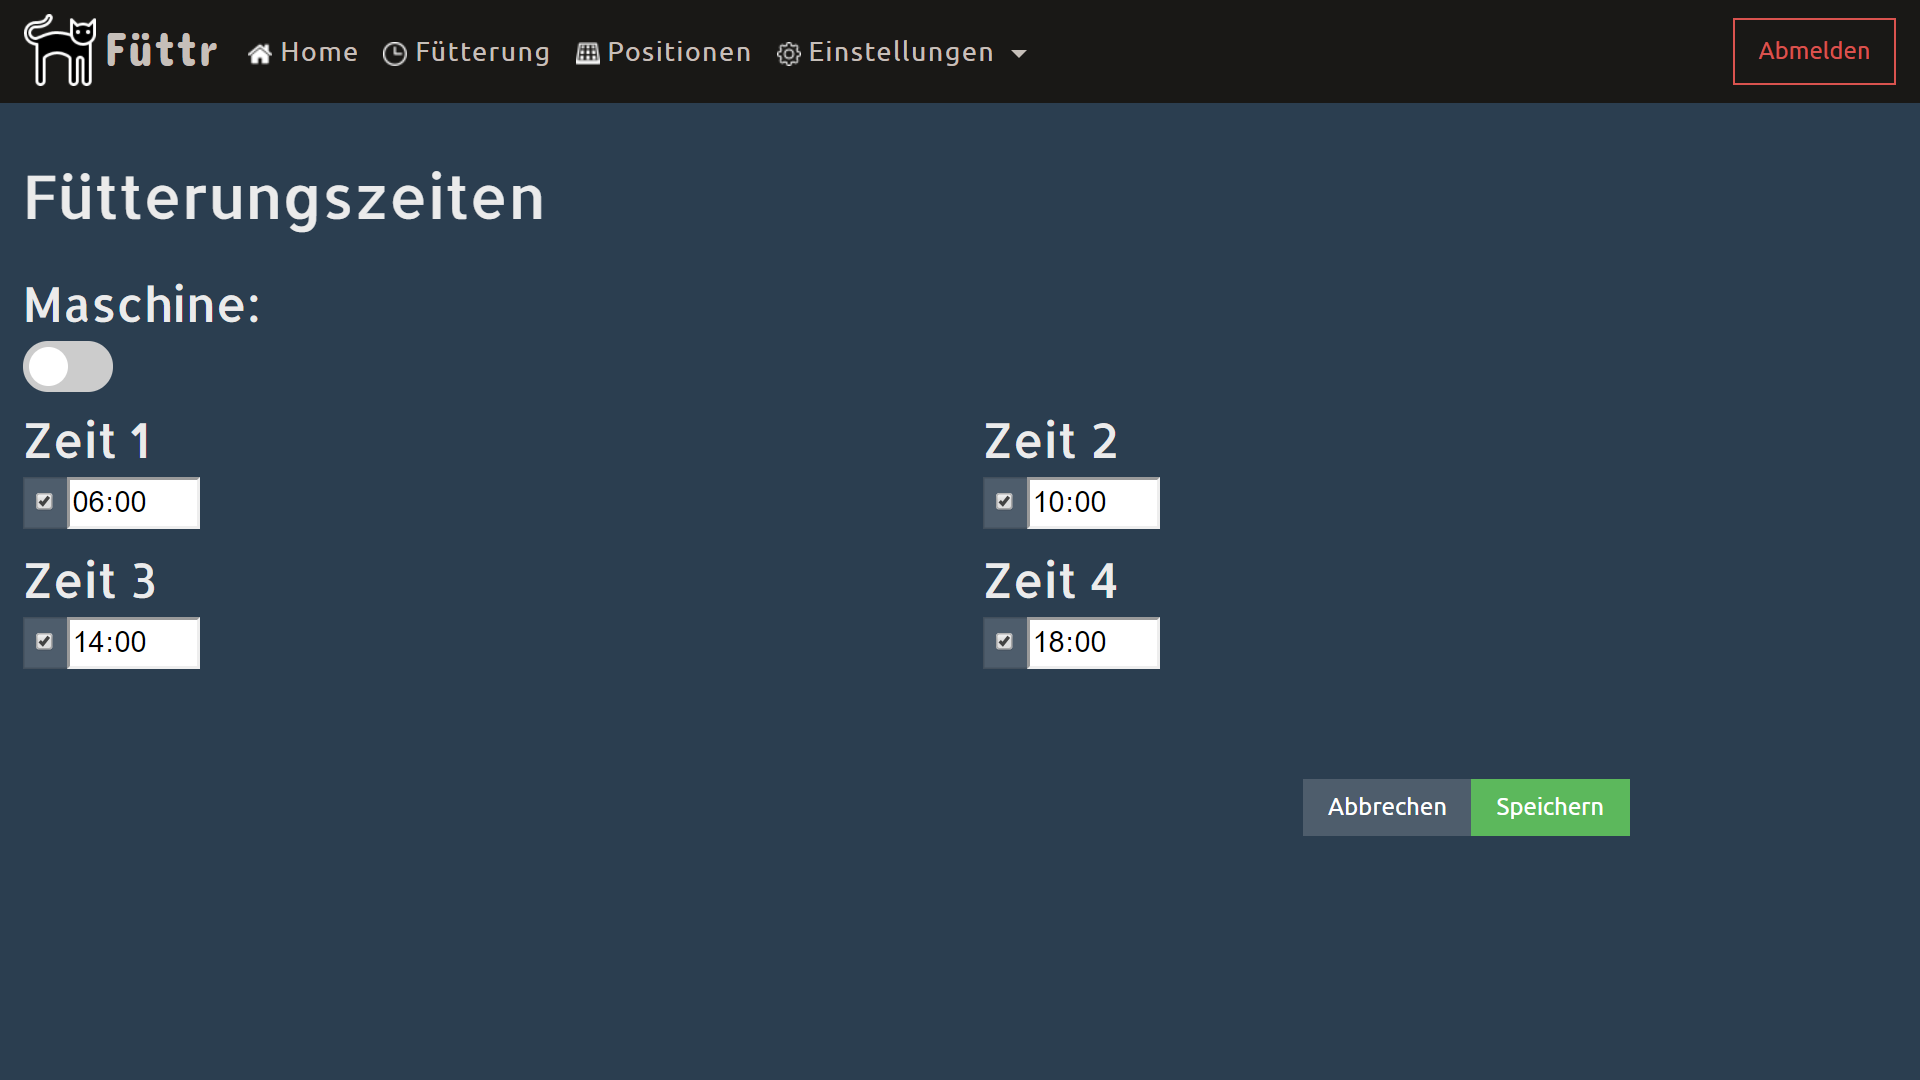
\includegraphics[width=0.65\textwidth]{Bilder/Greistorfer/Fuetterungszeiten}
  \end{center}
  \caption{Fütterungszeiten}
  \label{Fütterungszeiten}
  \vspace{-10pt}
\end{wrapfigure}

Auf der Fütterungszeiten-Seite kann der Benutzer die Katzenfütterungsanlage ein und ausschalten. Dies wurde mit einer Checkbox realisiert, die durch Styles wie ein Schalter gestaltet wurde. Darunter können die Fütterungszeiten geändert und deaktiviert werden. Siehe Abbildung \ref{Fütterungszeiten}. Der Button 'Speichern' wird deaktiviert, sobald eine Zeit ungültig eingegeben wurde, oder wenn die Zeiten nicht in aufsteigender Reihenfolge sortiert sind. \\

\begin{wrapfigure}{r}{0.7\textwidth}
\vspace{-10pt}
  \begin{center}
    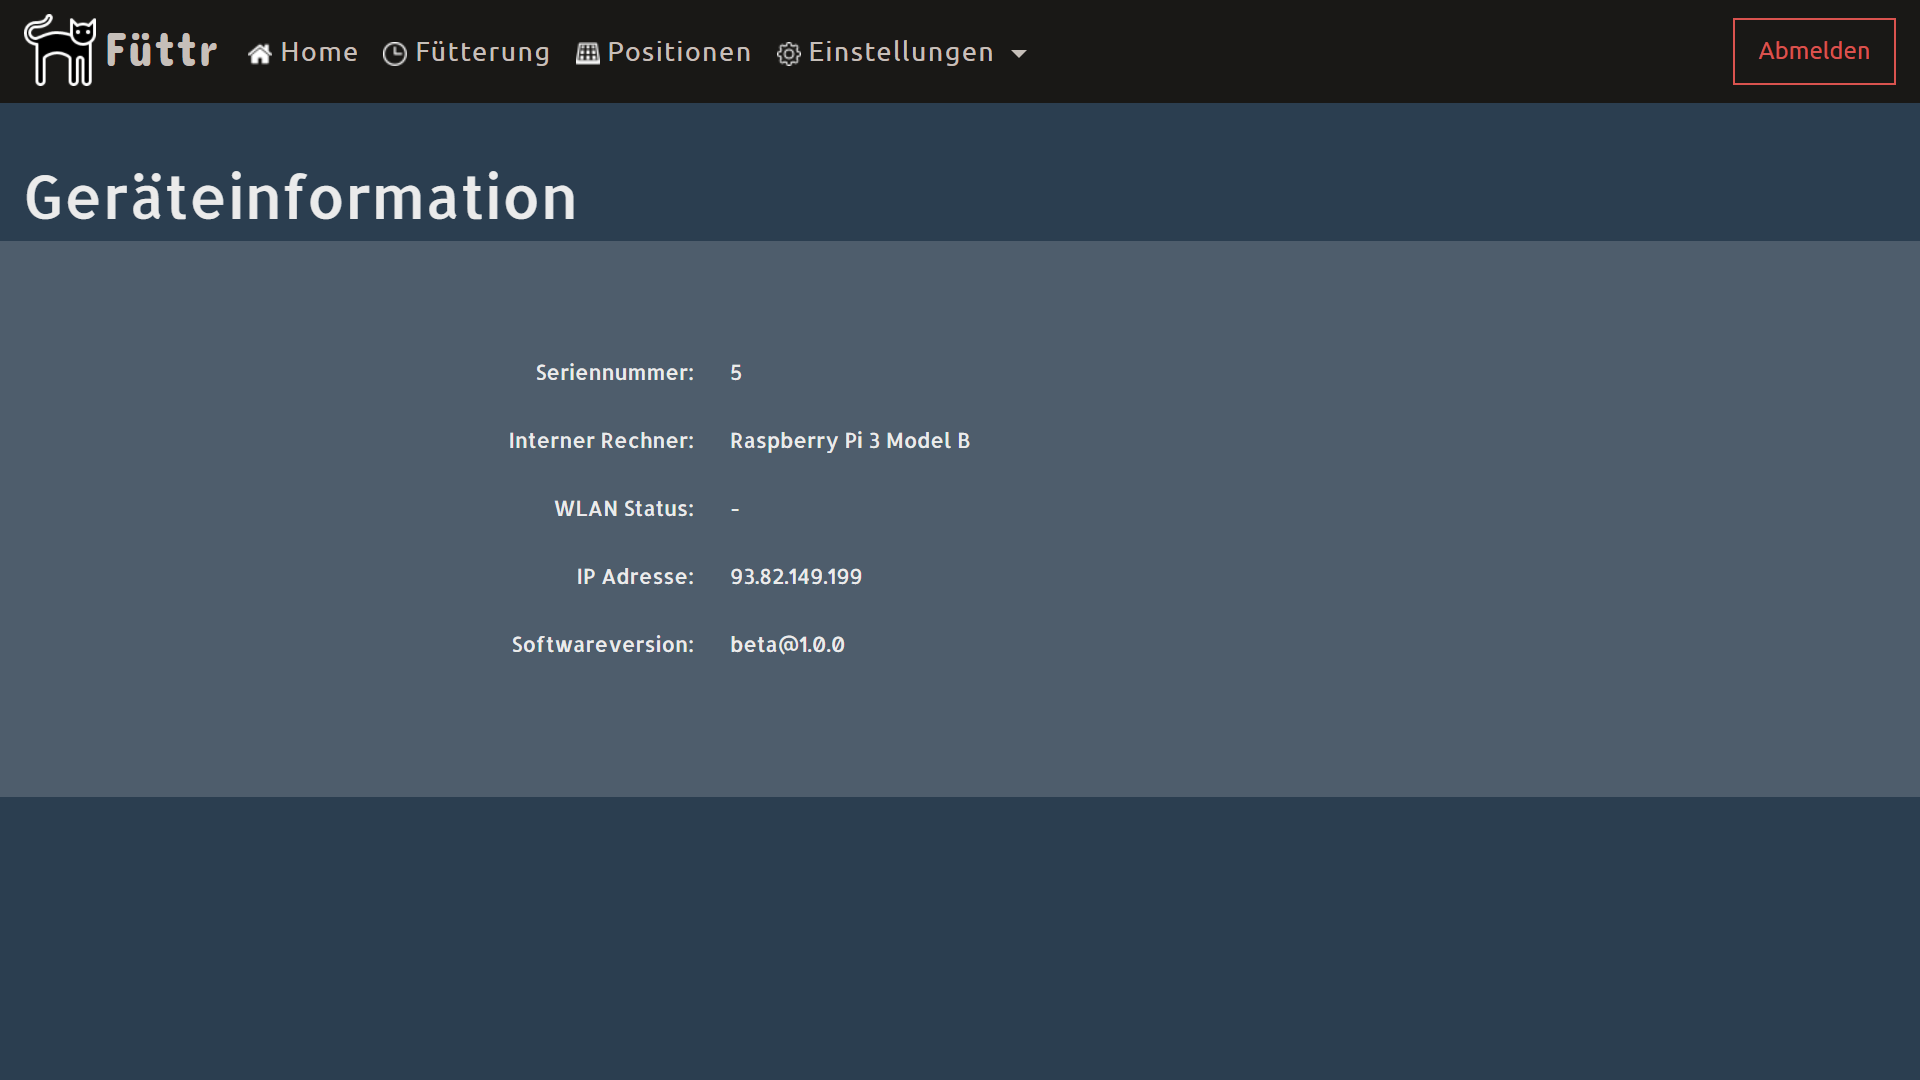
\includegraphics[width=0.65\textwidth]{Bilder/Greistorfer/Gerateinformation}
  \end{center}
  \caption{Geräteinformationen}
  \label{Geräteinformationen}
  \vspace{-60pt}
\end{wrapfigure}

Auf der Geräteinformations-Seite werden die wichtigsten Daten über das Gerät angezeigt. diese Daten sind:
\begin{itemize}
\item[•]Seriennummer
\item[•]Interner Rechner
\item[•]WLAN Status
\item[•]IP Adresse
\item[•]Softwareversion
\end{itemize}
Die IP-Adresse ist die aktuelle \textbf{externe} IP-Adresse. \newpage

\begin{wrapfigure}{r}{0.7\textwidth}
\vspace{-10pt}
  \begin{center}
    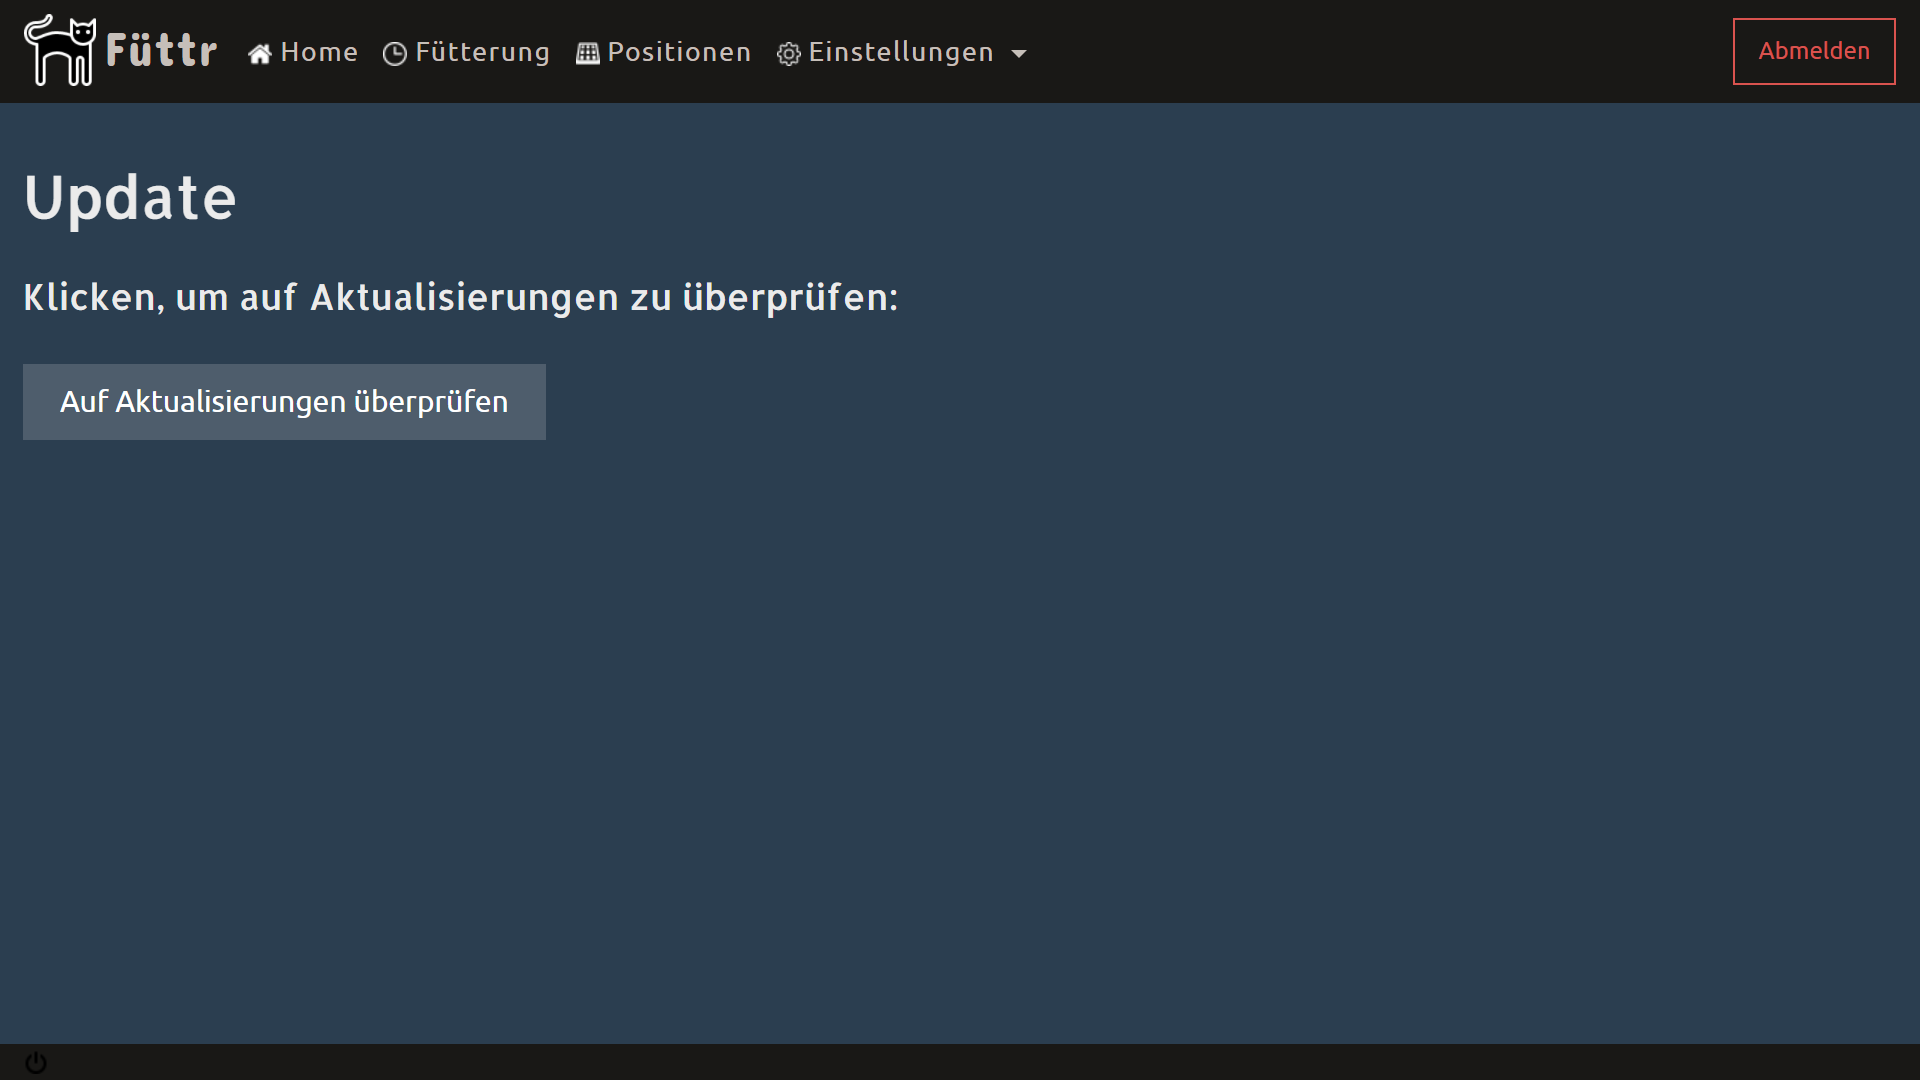
\includegraphics[width=0.65\textwidth]{Bilder/Greistorfer/Update}
  \end{center}
  \caption{Update}
  \label{Update}
  \vspace{-10pt}
\end{wrapfigure}

Auf der Update-Seite kann der Benutzer nach Updates suchen, Updates starten oder die Maschine herunterfahren. Wenn der Benutzer auf den Herunterfahren-Button klickt, der sich auf der linken Seite ganz unten befindet, wird er gewarnt, dass die Maschine nur mehr über das Aus- und wieder Einstecken des Netzteils Startbar ist.\\

\subsubsection{Funktion}
\label{sec:ums-client-funktion}

\paragraph*{Struktur} \mbox {}\\
Der Haupt-\textit{Component}, der geladen wird, wenn die Seite aufgerufen wird, ist \textit{app.component}. In seinem Template ist die Navigationsleiste, die sich alle Seiten teilen. Alle weiteren Seiten werden im \inlinecode{html}{<router-outlet></router-outlet>} angezeigt. Das ist ein \ac{HTML}-Tag der von Angulars Router zur Verfügung gestellt wird. Ein Router ist ein Service, dass das Navigieren der Seite ermöglicht. Damit das funktioniert, muss dem Router mitgeteilt werden, wie die Seite aufgebaut ist. Dies geschieht im \textit{router.module}:

\begin{lstlisting}[caption=Routes Definition,style=TS]
const routes: Routes = [
  { path: 'home', component: HomeComponent, 
  		data: { title: 'Füttr' }, canActivate: [AuthGuard]},
  { path: '', pathMatch: 'full', redirectTo: 'login'},
  { path: 'login', component: LoginComponent,
  		data: { title: 'Füttr - Login' }},
  { path: 'position', component: PositionComponent, 
  		data: { title: 'Füttr - Positions' }, canActivate: [AuthGuard]},
  { path: 'feed', component: FeedComponent, 
  		data: { title: 'Füttr - Feeding-Cycle' }, canActivate: [AuthGuard},
  { path: 'info', component: InfoComponent, 
  		data: { title: 'Füttr - Info' }, canActivate: [AuthGuard]},
  { path: 'update', component: UpdateComponent, 
  		data: { title: 'Füttr - Update' }, canActivate: [AuthGuard]},
  { path: '**', component: Error404Component, 
  		data: { title: 'Füttr - 404 (not found)'}}
];
\end{lstlisting}

Jede Route bekommt ein data Objekt übergeben, dass bei Aufruf der \textit{Component} dem @Input Decorator injiziert wird. Der jeweilige \textit{Component} ändert damit den Titel der Seite. Alle Routes, bis auf \textit{login} und \textit{404} sind von einem AuthGuard geschützt, dass bedeutet, nur authorisierte Benutzer können diese Routes aufrufen. Der Request auf \textit{root} \inlinecode{TS}{path: ''} wird umgeleitet auf \textit{login}. Für jeden Request, dessen Route nicht definiert ist, wird der 404 Component geladen: \inlinecode{TS}{path: '**'}.

\paragraph*{\ac{HTTP} Service}\mbox{}\\
Da alle \textit{Components} Daten vom Server holen und manche auch Daten zum Server schicken, war es die logische Schlussfolgerung, ein Service zu erstellen, das egal welche Art von \ac{HTTP} Anfrage verarbeiten kann. Dieses Service ist \textit{http.service}. Alle Anfragen, egal ob \textit{GET} oder \textit{PUT} werden von diesem Service getätigt. Das Service importiert Angular's \textit{HttpClient}, mit dem es sehr einfach ist, Anfragen zu erstellen und die Antworten zu verarbeiten. Die Antworten vom Server sind vom Typ \textit{application/json}, das bedeutet, sie sind \ac{JSON}-Dateien, die der \textit{HttpClient} dann in Objekte umwandelt. Diese Objekte werden dem \textit{Component} übergeben, sobald die Anfrage abgeschlossen wurde.

\paragraph*{Fütterungszeiten}\mbox{}\\
Die Eingabe wurde realisiert durch \ac{HTML} input Elemente vom Typ \textit{time}. Da \textit{time} Browserabhängig ist und ältere Browser es als \textit{text} interpretieren könnten, und die Application auf allen Browsern funktionieren soll, werden alle Eingabefelder auf Richtigkeit überprüft. Außerdem sollen alle Zeiten in aufsteigender Reihenfolge eingegeben werden. Der \textit{time} Typ ist eigentlich nur ein string, das bedeutet, um die Reihenfolge zu überprüfen, müssen diese zuerst in Zahlen umgewandelt werden. Das geht mit der Funktion \inlinecode{TS}{parseInt()}. Ein string von einem \textit{time} input sieht meistens so aus: \inlinecode{TS}{'12:34'} Wenn die Zeit leer ist, sieht er so aus: \inlinecode{TS}{'--:--'} Auf diese beiden Arten muss unser Parser vorbereitet sein. Der Parser wandelt den string in Minuten um, danach werden sie verglichen. Sollte eine Zeit ungültig sein oder sollte eine Zeit ausser Reihenfolge sein, so wird der Speicher-Button deaktiviert. Überprüft wird, sobald der User etwas ändert. Dies geschieht durch den DoCheck() Lifecycle Hook (siehe \ref{sec:ang-components}). Über den Fütterungszeiten kann man außerdem die Maschine ein und ausschalten. Dies ist realisiert durch eine Checkbox, die mit \ac{CSS} wie ein Schalter gestyled wurde.

\begin{lstlisting}[caption=Zeiten Parser,style=TS,label=zeiten_parser,captionpos=t]
toMinutes(time: string): number {
  let timeHours: number;
  let timeMinutes: number;
  if (time[0] === '-' && time[1] === '-' 
      && time[3] === '-' && time[4] === '-') {
    return null;
  }
  timeHours = parseInt(time[0], 10) * 10;
  timeHours = timeHours + parseInt(time[1], 10);
  timeMinutes = parseInt(time[3], 10) * 10;
  timeMinutes = timeMinutes + parseInt(time[4], 10);
  return timeHours * 60 + timeMinutes;
}
\end{lstlisting}

\paragraph*{Updates}\mbox{}\\
Auf der Updates Seite kann der Benutzer nach neuen Updates suchen und das Gerät updaten. Realisiert wurde dies durch eine Anfrage an Github, wo eine Datei namens \textit{version.json} liegt. Diese wird verglichen mit der Datei, die auf dem System liegt. Dieser Vergleich geschieht bereits im OnInit() Lifecycle Hook (siehe \ref{sec:ang-components}). Der User kann nochmal nach Updates suchen, wenn er dies möchte. Sollte ein Update verfügbar sein, so wird der Button aktiv und der Benutzer kann sich dazu entscheiden, dass Gerät upzudaten. Wird aktualisiert, so wird eine Anfrage an den Server gesendet siehe \ref{sec:ums-server-funktion}. Der Client beginnt, dauerhaft Anfragen zu senden, bis eine fehlschlägt. Eine Nachricht teilt dem Benutzer mit, dass das System aktualisiert. Dann werden so lange Anfragen gesendet, bis wieder eine Antwort ankommt. Dann wird die Seite automatisch neu geladen. Der Updatevorgang ist damit abgeschlossen.

\subsection{Server}
\label{sec:ums-server}

\subsubsection{Serverpfade}
\label{sec:ums-server-pfade}

\paragraph*{GET}\mbox{}\\
\begin{forest}
	[\textit{root}
		[api
			[version]
			[callMeMaybe]
			[getUpdate]
			[shutdown]
			[ip]		
		]
		[de]
		[en]
	]
\end{forest}

\paragraph*{POST}\mbox{}\\
\begin{forest}
	[\textit{root}
		[api
			[putMeHere]	
		]
		[login]
		[logout]	
	]
\end{forest}


\subsubsection{Funktion}
\label{sec:ums-server-funktion}
Ich Spasst schreibe hiermit meine blumenhafte Diplomarbeit. Viel Hass steht dahinter und auch keine Liebe. In Liebe, Spasst.


\subsubsection{Mongodb}
\label{sec:ums-server-mongo}


\subsubsection{Kommunikation mit dem Java Programm}
\label{sec:ums-server-java}


\section{Zusammenfassung und Verbesserungsmöglichkeiten}
\label{sec:zusammenfassung}
